\documentclass[12pt]{article}
\usepackage[T1]{fontenc}
\usepackage{indentfirst}
\usepackage{listings}
\usepackage{color}
\usepackage{hyperref}
\usepackage{caption}
\usepackage{graphicx}
\usepackage{float}
\captionsetup[table]{name=Tabela}
\renewcommand{\figurename}{Wyk.}
\lstset{numbers=left, language=Python, breaklines=true, mathescape=true, frame=tB, numberstyle=\tiny, basicstyle=\scriptsize, keywordstyle=\color{black}\bfseries\em, keywords={,return,in,if,else,to,do,foreach,while,begin,end}, xleftmargin=.04\textwidth}
\setlength{\parskip}{1em}
\renewcommand{\contentsname}{Spis treści}
\author{Franciszek Magiera, Dawid Lech}
\title{Wykorzystanie algorytmu genetycznego w rozwiązywaniu problemu QAP.}
\date{09.01.2019}
\begin{document}
\sloppy
\maketitle
\newpage
\tableofcontents
\newpage
\section{Wstęp}
Naszym zadaniem było znalezienie takiego rozmieszczenia fabryk, znając przepływ materiałów oraz odległości między nimi, aby energia potrzebna do transportu materiałów była minimalna. Jest to przypadek NP-trudnego problemu QAP. Rozwiązania problemu poszukiwaliśmy przy pomocy algorytmu genetycznego.
\section{Model matematyczny}
Mamy dany zbiór n fabryk oraz n dostępnych na budowę miejsc, które numerujemy od 1 do n. Dana jest również macierz przepływu $n\times n$, której element w i-tej kolumnie i j-tym wierszu oznacza ilość transportowanych materiałów z fabryki oznaczonej numerem i do fabryki oznaczonej numerem j oraz symetryczną macierz odległości pomiędzy poszczególnymi miejscami, również o wymiarach $n\times n$, której element w i-tej kolumnie i j-tym wierszu oznacza odległość miejsca oznaczonego numerem i od miejsca oznaczonego numerem j (w obydwu przypadkach $i,j \in [1,n]$). Rozwiązania problemu szukamy w postaci n-elementowej permutacji, gdzie element na i-tym miejscu o wartości j oznacza przyporządkowanie fabryki o j-tym numerze na miejsce o i-tym numerze.
\par
Oznaczając macierz przepływu materiałów pomiędzy fabrykami przez W, macierz odległości pomiędzy dostępnymi miejscami przez D oraz permutację będącą rozwiązaniem poprzez s, funkcję celu możemy zapisać w postaci:
\begin{equation}
F(s) = \sum_{i=1}^{n}  \sum_{j=1}^{n}D_{i,j}W_{s(i), s(j)} \longrightarrow min \label{Funkcja celu}
\end{equation}
W przypadku symetrycznych macierzy przepływu możnaby zmodyfikować powyższą funkcję dzieląc ją przez 2, bądź rozpoczynając drugie sumowanie od j=i do n, co skróciłoby czas potrzebny na obliczenie wartości funkcji celu.
\section{Opis algorytmu}
Aby znaleźć optymalne rozwiązanie opisanego problemu, przeszukujemy przestrzeń dopuszczalnych rozwiazań. Korzystamy przy tym z algorytmu genetycznego, należącego do szerszej klasy algorytmów ewolucyjnych. Algorytm genetyczny wymaga odpowiedniej reprezentacji przestrzeni rozwiązań, dla której elementów łatwo jest wykonać proste operacje krzyżowania, mutacji itp. oraz funkcji celu, co sprawia, że dobrze nadaje się do rozwiązania naszego problemu. \par
Algorytmy genetyczne wykorzystują mechanizmy zainspirowane ewolucją biologiczną takie jak krzyżowanie, mutacja czy selekcja. Przykładowe rozwiązanie problemu można skojarzyć z osobnikiem należącym do populacji (zbioru kilku rozwiązań). Funkcję celu można rozumieć jako miarę przystosowania danego osobnika - determinuje ona jakość rozwiązania. Populacja początkowa jest generowana losowo. Ewolucja populacji zachodzi po wielokrotnym stosowaniu wcześniej wymienionych mechanizmów. W efekcie z każdą generacją uzyskujemy coraz to lepiej przystosowaną populację (składającą sie z osobników o niższych wartościach funkcji celu). \par
Potencjalnym problemem na jaki można się natknąć wykorzystując algorytm genetyczny jest zbyt szybkie osiąganie jednolitej populacji. Z jednej strony prowadzi to do szybkiego znalezienia rozwiązania, jednak najczęściej jest ono jedynie optimum lokalnym dalekim od rozwiązania optymalnego. Aby uniknąć tego problemu należy zadbać o losowość działania algorytmu np. poprzez dodanie mutacji oraz stosować techniki selekcji, które utrzymują zróżnicowaną populację. \par
Czynnikami limitującymi stosowanie algorytmów genetycznych jest złożoność funkcji celu, która musi być wielokrotnie obliczana podczas wykonania algorytmu oraz rozmiar problemu do którego silni proporcjonalny jest rozmiar przestrzeni rozwiązań. \par
Należy również pamiętać, że algorytmy genetyczne to metody przybliżone, co oznacza, że nie mamy pewności co do tego czy znalezione przez nas rozwiązanie jest optymalne, a nawet jeśli takie znaleźliśmy, to nie możemy tego stwierdzić. \par
Stworzony przez nas algorytm podąża według następującego schematu: wczytujemy parametry algorytmu takie jak prawdopodobieństwo mutacji i rodzaj operatorów oraz populację startową z pliku. Następnie w pętli wykonujemy kolejno selekcji n rodziców z dotychczasowej populacji, następnie n razy wybieramy losowo dwóch rodziców, których krzyżujemy ze sobą. Ich potomków z pewnym prawdopodobieństwem mutujemy, a następnie korzystając z operatora sukcesji wybieramy osobników, którzy przechodzą do następnej populacji (kolejnej generacji). Pętlę zatrzymujemy po wykonaniu okrelślonej ilości iteracji bądź gdy nie uzyskamy polepszenia wartości najlepszego globalnie rozwiązania przez kilka iteracji. Schemat ten przedstawiamy w postaci pseudokodu na listingu 1.
\begin{lstlisting}[caption={Pseudokod głównego programu}]
[operator_selekcji, operator_krzyzowania, prawdopodobienstwo_mutacji, operator_mutacji, operator_sukcesji, liczba_rodzicow, limit_iteracji, limit, populacja] = wczytaj_parametry(sciezka_do_pliku)
i = 0
j = 0 # ilosc iteracji bez poprawy wartosci najlepszego globalnie rozwiazania
dzieci = []
dzieci.length = liczba_rodzicow * (liczba_rodzicow - 1)
najlepsi = []
najlepsi.length = max(limit_iteracji, limit)
while i < limit_iteracji and j < limit do
	i = i + 1
	rodzice = operator_selekcji(populacja)
	for k = 1 to rodzice.length do
		x = random(1, rodzice.length)
		y = random(1, rodzice.length)
		[dziecko1, dziecko2] = operator_krzyzowania(rodzice[x], rodzice[y])
		dzieci.append(dziecko1)
		dzieci.append(dziecko2)
	for k = 1 to rodzice.length do
		if random(0,1) < prawdopodobienstwo_mutacji then
			dzieci[i] = operator_mutacji(dzieci[i])
	populacja = operator_sukcesji(populacja.length, dzieci, rodzice)
	najlepsze[i] = min(populacja, key=funkcja_celu)
	if (i == 1) then
		globalnie_najlepsze = najlepsze[i]
	else if globalnie_najlepsze > najlepsze[i] then
		globalnie_najlepsze = najlepsze[i]
	if globalnie_najlepsze <= najlepsze[i] then
		j += 1
\end{lstlisting}
\section{Oprogramowanie}
Algorytm zaimplementowaliśmy w języku programowania Python. Wszystkie skrypty napisaliśmy w jego najnowszej wersji 3.7. Stworzyliśmy funkcje realizujące operatory selekcji proporcjonalnej, turniejowej oraz odcinającej, operatory krzyżowania PMX oraz OX, operatory mutacji typu swap, inversion, scramble. Skorzystaliśmy również z biblioteki Numpy do obliczeń numerycznych, aby program działał szybciej, oraz z biblioteki Matplotlib do rysowania wykresów. Dane takie jak macierze przepływów przechowujemy w plikach csv, ponieważ łatwo można z nich odczytywać dane, a także edytować je przy pomocy innych programów, na przykład arkuszy kalkulacyjnych. Dane konfiguracyjne zawierające ustawienia według jakich algorytm ma działać (np. rodzaj operatora krzyżowania, prawdopodbieństwo mutacji, macierz przepływu itp.) zapisaliśmy w zwykłym pliku tekstowym (.txt). Dzięki temu moglimśmy łatwo testować działanie naszego algortymu z różnymi parametrami oraz danymi. Cały projekt można pobrać z repozytorium znajdującym się pod linkiem \url{https://github.com/franekmagiera/algorytm-genetyczny-mmwd}. Do uruchomienia skryptów potrzebny jest komputer z zainstalowanym interpreterem języka Python w wersji 3.7. \par
Aby uruchomić algorytm, należy najpierw w pliku input\textunderscore data.txt określić rządane parametry algorytmu oraz dodać ścieżki do miejsc w których znajdują się macierz przepływu, populacja początkowa oraz macierz odległości. Losową populację początkową można również wygenerować przy pomocy skryptu generate\textunderscore new\textunderscore population.py (trzeba wówczas określić w skrypcie wymiary populacji początkowej). Następnie można uruchomić skrypt algorithm\textunderscore v3.py. Po wykonaniu się programu na ekran wypisywane jest znalezione najlepsze rozwiązanie, jego wartość funkcji celu oraz wykres przebiegu działania algorytmu na którym znajduje się najgorsze i najlepsze rozwiązanie w danej iteracji oraz globalnie najlepsze rozwiązanie.
\section{Testy}
Początkowo przetestowaliśmy nasz algorytm dla danych przedstawionych w tabeli 1 oraz 2.
\begin{table}[H]
\caption{Macierz przepływu}
\begin{center}
	\begin{tabular}{| c | c | c | c | c | c | c | c | c |}
		\hline
0&2&4&0&0&0&2&0&0\\ \hline
2&0&3&1&0&6&0&0&2\\ \hline
4&3&0&0&0&3&0&0&0\\ \hline
0&1&0&0&1&0&1&2&0\\ \hline
0&0&0&1&0&0&0&0&0\\ \hline
0&6&3&0&0&0&0&0&2\\ \hline
2&0&0&1&0&0&0&4&3\\ \hline
0&0&0&2&0&0&4&0&0\\ \hline
0&2&0&0&0&2&3&0&0\\ \hline
	\end{tabular}
\end{center}
\end{table}
\begin{table}[H]
\caption{Macierz odległości}
\begin{center}
	\begin{tabular}{| c | c | c | c | c | c | c | c | c | c | c | c | c |}
		\hline
0&32&68&97&75&70&75&40&24\\ \hline
32&0&42&80&53&65&82&47&29\\ \hline
68&42&0&45&15&49&79&55&50\\ \hline
97&80&45&0&30&36&65&65&73\\ \hline
75&53&15&30&0&38&69&53&53\\ \hline
70&65&49&36&38&0&31&32&46\\ \hline
75&82&79&65&69&31&0&36&56\\ \hline
40&47&55&65&53&32&36&0&19\\ \hline
24&29&50&73&53&46&56&19&0\\ \hline
	\end{tabular}
\end{center}
\end{table}
Dane zaczerpnęliśmy ze strony \url{https://neos-guide.org/content/qap9} Uniwersytetu Wisconsin-Madison. Wybraliśmy stosunkowo niewielki problem o rozmiarach macierzy $9 \times 9$, ponieważ celem pierwszego testu było jedynie sprawdzenie poprawności działania naszej implementacji algorytmu. Jak widać z przebiegu na wykresie 1, wartość funkcji celu najlepszego rozwiązania szybko stabilizuje się, bo tylko po około 20 iteracjach. Udało nam się uzyskać satysfakcjonujące wyniki, w szczególności na wykresie 1 znajduje się przebieg algorytmu dający w wyniku rozwiązanie optymalne postaci $(2, 0, 8, 7, 6, 3, 4, 5, 1)$ o wartości funkcji celu równej 1160.
\begin{figure}[H]
\caption{Przebieg działania algorytmu dla problemu zawartego w tabelach 1 i 2}
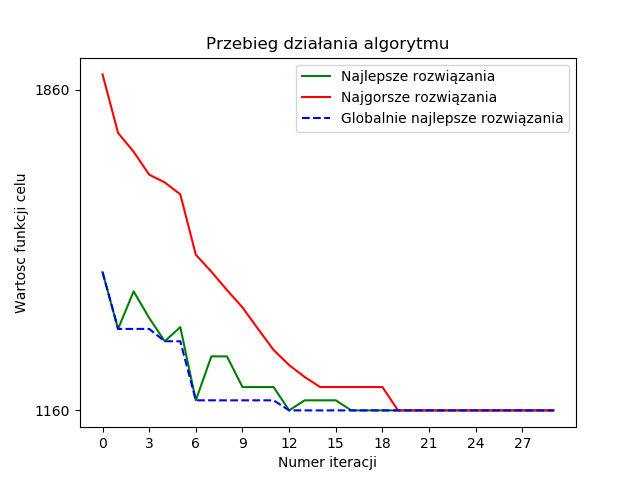
\includegraphics{najlepsze9x9.png}
\end{figure}
\par
Następnie przetestowaliśmy działanie naszego algorytmu dla większych danych z macierzami kosztów i odległości o rozmiarach $36 \times 36$. Dane przedstawione w tabelach 3 i 4 zaczerpnęliśmy z biblioteki problemów QAP dostępnej na stronie internetowej pod adresem \url{http://anjos.mgi.polymtl.ca/qaplib/}. Pochodzą one z pracy L. Steinberga - The Backboard wiring problem: a placement algorithm. \textit{SIAM Review}, 3:37-50, 1961 i dotyczą problemu rozmieszczenia komponentów elektronicznych w celu minimalizacji zużytej energii elektrycznej. Odległości zostałe podane w przestrzeni metrycznej Manhattan. Wartość funkcji celu optymalnego rozwiązania wynosiła 9526.
\begin{table}[H]
\caption{Macierz kosztów}
\footnotesize
\tabcolsep=0.11cm
\begin{center}
\scalebox{0.7}{
	\begin{tabular}{| c | c | c | c | c | c | c | c | c | c | c | c | c | c | c | c | c | c | c | c | c | c | c | c | c | c | c | c | c | c | c | c | c | c | c | c | c | c |}
		\hline
0&0&0&2&1&7&9&0&4&75&7&12&22&7&1&0&0&0&0&23&0&0&0&0&0&0&0&0&0&0&0&0&0&0&0&0\\ \hline
0&0&0&0&0&0&4&16&0&8&0&0&16&0&0&0&0&6&0&4&0&0&0&0&0&0&0&0&0&0&0&0&0&0&0&0\\ \hline
0&0&0&0&0&4&16&20&0&0&0&0&20&0&0&0&0&0&0&4&0&0&0&0&0&0&0&0&0&0&0&0&0&0&0&0\\ \hline
2&0&0&0&29&5&18&47&23&2&4&0&48&0&4&0&0&0&0&25&0&0&0&0&0&0&0&0&0&0&0&0&0&0&0&0\\ \hline
1&0&0&29&0&18&12&25&0&0&4&0&25&0&3&0&0&0&0&18&0&3&0&0&0&0&0&0&0&0&0&0&0&0&0&0\\ \hline
7&0&4&5&18&0&4&2&0&1&23&2&19&0&0&0&0&0&2&19&0&0&0&0&0&0&0&0&0&0&0&0&0&0&0&0\\ \hline
9&4&16&18&12&4&0&0&14&72&7&8&39&8&40&8&0&8&4&7&0&0&0&0&0&0&0&28&8&0&0&0&0&0&0&0\\ \hline
0&16&20&47&25&2&0&0&10&71&2&0&0&0&0&0&0&41&0&0&0&0&0&0&0&0&7&8&0&0&0&0&0&0&0&0\\ \hline
4&0&0&23&0&0&14&10&0&14&0&0&18&0&0&0&0&0&0&0&0&0&0&0&0&0&0&0&0&0&0&0&0&0&0&0\\ \hline
75&8&0&2&0&1&72&71&14&0&11&1&17&0&1&0&0&17&0&15&0&0&0&0&0&0&0&0&0&0&0&0&0&0&0&0\\ \hline
7&0&0&4&4&23&7&2&0&11&0&316&33&8&2&0&0&0&8&34&0&0&6&0&0&0&10&0&0&6&0&0&0&0&0&0\\ \hline
12&0&0&0&0&2&8&0&0&1&316&0&157&25&4&0&0&1&0&0&0&0&0&0&22&0&1&0&0&0&0&0&0&0&0&0\\ \hline
22&16&20&48&25&19&39&0&18&17&33&157&0&11&6&0&0&6&0&5&8&3&10&0&0&0&9&11&2&0&0&1&0&0&0&0\\ \hline
7&0&0&0&0&0&8&0&0&0&8&25&11&0&3&0&0&1&1&21&0&1&0&2&0&0&5&0&0&3&2&5&5&4&0&0\\ \hline
1&0&0&4&3&0&40&0&0&1&2&4&6&3&0&19&0&2&2&12&0&0&0&0&0&0&0&7&3&0&0&0&0&0&0&0\\ \hline
0&0&0&0&0&0&8&0&0&0&0&0&0&0&19&0&0&6&0&1&0&0&0&0&0&0&0&0&0&0&0&0&0&0&0&0\\ \hline
0&0&0&0&0&0&0&0&0&0&0&0&0&0&0&0&0&40&0&0&0&0&0&0&0&0&0&0&0&0&0&0&0&0&0&0\\ \hline
0&6&0&0&0&0&8&41&0&17&0&1&6&1&2&6&40&0&0&26&0&0&0&0&0&0&0&0&0&0&0&0&0&0&0&0\\ \hline
0&0&0&0&0&2&4&0&0&0&8&0&0&1&2&0&0&0&0&13&9&0&7&0&0&0&0&27&16&3&0&20&0&4&0&0\\ \hline
23&4&4&25&18&19&7&0&0&15&34&0&5&21&12&1&0&26&13&0&11&4&36&0&0&0&16&18&9&10&1&28&6&2&0&0\\ \hline
0&0&0&0&0&0&0&0&0&0&0&0&8&0&0&0&0&0&9&11&0&36&6&0&8&0&2&0&0&0&0&0&0&0&0&0\\ \hline
0&0&0&0&3&0&0&0&0&0&0&0&3&1&0&0&0&0&0&4&36&0&0&0&0&0&4&0&0&0&0&0&0&0&0&0\\ \hline
0&0&0&0&0&0&0&0&0&0&6&0&10&0&0&0&0&0&7&36&6&0&0&0&0&12&9&0&0&0&0&0&0&0&0&0\\ \hline
0&0&0&0&0&0&0&0&0&0&0&0&0&2&0&0&0&0&0&0&0&0&0&0&26&0&5&0&0&0&0&0&0&0&0&0\\ \hline
0&0&0&0&0&0&0&0&0&0&0&22&0&0&0&0&0&0&0&0&8&0&0&26&0&35&2&0&0&0&0&0&0&0&0&0\\ \hline
0&0&0&0&0&0&0&0&0&0&0&0&0&0&0&0&0&0&0&0&0&0&12&0&35&0&4&0&0&0&0&0&0&0&0&0\\ \hline
0&0&0&0&0&0&0&7&0&0&10&1&9&5&0&0&0&0&0&16&2&4&9&5&2&4&0&0&0&0&0&0&0&0&0&0\\ \hline
0&0&0&0&0&0&28&8&0&0&0&0&11&0&7&0&0&0&27&18&0&0&0&0&0&0&0&0&10&22&4&6&4&12&0&0\\ \hline
0&0&0&0&0&0&8&0&0&0&0&0&2&0&3&0&0&0&16&9&0&0&0&0&0&0&0&10&0&19&12&0&0&0&0&0\\ \hline
0&0&0&0&0&0&0&0&0&0&6&0&0&3&0&0&0&0&3&10&0&0&0&0&0&0&0&22&19&0&19&4&5&8&0&0\\ \hline
0&0&0&0&0&0&0&0&0&0&0&0&0&2&0&0&0&0&0&1&0&0&0&0&0&0&0&4&12&19&0&0&3&13&0&0\\ \hline
0&0&0&0&0&0&0&0&0&0&0&0&1&5&0&0&0&0&20&28&0&0&0&0&0&0&0&6&0&4&0&0&18&24&0&0\\ \hline
0&0&0&0&0&0&0&0&0&0&0&0&0&5&0&0&0&0&0&6&0&0&0&0&0&0&0&4&0&5&3&18&0&20&0&0\\ \hline
0&0&0&0&0&0&0&0&0&0&0&0&0&4&0&0&0&0&4&2&0&0&0&0&0&0&0&12&0&8&13&24&20&0&0&0\\ \hline
0&0&0&0&0&0&0&0&0&0&0&0&0&0&0&0&0&0&0&0&0&0&0&0&0&0&0&0&0&0&0&0&0&0&0&0\\ \hline
0&0&0&0&0&0&0&0&0&0&0&0&0&0&0&0&0&0&0&0&0&0&0&0&0&0&0&0&0&0&0&0&0&0&0&0\\ \hline
	\end{tabular}}
\end{center}

\end{table}
\begin{table}[H]
\caption{Macierz odległości}
\footnotesize
\begin{center}
\scalebox{0.7}{
	\begin{tabular}{| c | c | c | c | c | c | c | c | c | c | c | c | c | c | c | c | c | c | c | c | c | c | c | c | c | c | c | c | c | c | c | c | c | c | c | c | c | c |}
		\hline
0&1&2&3&4&5&6&7&8&1&2&3&4&5&6&7&8&9&2&3&4&5&6&7&8&9&10&3&4&5&6&7&8&9&10&11\\ \hline
1&0&1&2&3&4&5&6&7&2&1&2&3&4&5&6&7&8&3&2&3&4&5&6&7&8&9&4&3&4&5&6&7&8&9&10\\ \hline
2&1&0&1&2&3&4&5&6&3&2&1&2&3&4&5&6&7&4&3&2&3&4&5&6&7&8&5&4&3&4&5&6&7&8&9\\ \hline
3&2&1&0&1&2&3&4&5&4&3&2&1&2&3&4&5&6&5&4&3&2&3&4&5&6&7&6&5&4&3&4&5&6&7&8\\ \hline
4&3&2&1&0&1&2&3&4&5&4&3&2&1&2&3&4&5&6&5&4&3&2&3&4&5&6&7&6&5&4&3&4&5&6&7\\ \hline
5&4&3&2&1&0&1&2&3&6&5&4&3&2&1&2&3&4&7&6&5&4&3&2&3&4&5&8&7&6&5&4&3&4&5&6\\ \hline
6&5&4&3&2&1&0&1&2&7&6&5&4&3&2&1&2&3&8&7&6&5&4&3&2&3&4&9&8&7&6&5&4&3&4&5\\ \hline
7&6&5&4&3&2&1&0&1&8&7&6&5&4&3&2&1&2&9&8&7&6&5&4&3&2&3&10&9&8&7&6&5&4&3&4\\ \hline
8&7&6&5&4&3&2&1&0&9&8&7&6&5&4&3&2&1&10&9&8&7&6&5&4&3&2&11&10&9&8&7&6&5&4&3\\ \hline
1&2&3&4&5&6&7&8&9&0&1&2&3&4&5&6&7&8&1&2&3&4&5&6&7&8&9&2&3&4&5&6&7&8&9&10\\ \hline
2&1&2&3&4&5&6&7&8&1&0&1&2&3&4&5&6&7&2&1&2&3&4&5&6&7&8&3&2&3&4&5&6&7&8&9\\ \hline
3&2&1&2&3&4&5&6&7&2&1&0&1&2&3&4&5&6&3&2&1&2&3&4&5&6&7&4&3&2&3&4&5&6&7&8\\ \hline
4&3&2&1&2&3&4&5&6&3&2&1&0&1&2&3&4&5&4&3&2&1&2&3&4&5&6&5&4&3&2&3&4&5&6&7\\ \hline
5&4&3&2&1&2&3&4&5&4&3&2&1&0&1&2&3&4&5&4&3&2&1&2&3&4&5&6&5&4&3&2&3&4&5&6\\ \hline
6&5&4&3&2&1&2&3&4&5&4&3&2&1&0&1&2&3&6&5&4&3&2&1&2&3&4&7&6&5&4&3&2&3&4&5\\ \hline
7&6&5&4&3&2&1&2&3&6&5&4&3&2&1&0&1&2&7&6&5&4&3&2&1&2&3&8&7&6&5&4&3&2&3&4\\ \hline
8&7&6&5&4&3&2&1&2&7&6&5&4&3&2&1&0&1&8&7&6&5&4&3&2&1&2&9&8&7&6&5&4&3&2&3\\ \hline
9&8&7&6&5&4&3&2&1&8&7&6&5&4&3&2&1&0&9&8&7&6&5&4&3&2&1&10&9&8&7&6&5&4&3&2\\ \hline
2&3&4&5&6&7&8&9&10&1&2&3&4&5&6&7&8&9&0&1&2&3&4&5&6&7&8&1&2&3&4&5&6&7&8&9\\ \hline
3&2&3&4&5&6&7&8&9&2&1&2&3&4&5&6&7&8&1&0&1&2&3&4&5&6&7&2&1&2&3&4&5&6&7&8\\ \hline
4&3&2&3&4&5&6&7&8&3&2&1&2&3&4&5&6&7&2&1&0&1&2&3&4&5&6&3&2&1&2&3&4&5&6&7\\ \hline
5&4&3&2&3&4&5&6&7&4&3&2&1&2&3&4&5&6&3&2&1&0&1&2&3&4&5&4&3&2&1&2&3&4&5&6\\ \hline
6&5&4&3&2&3&4&5&6&5&4&3&2&1&2&3&4&5&4&3&2&1&0&1&2&3&4&5&4&3&2&1&2&3&4&5\\ \hline
7&6&5&4&3&2&3&4&5&6&5&4&3&2&1&2&3&4&5&4&3&2&1&0&1&2&3&6&5&4&3&2&1&2&3&4\\ \hline
8&7&6&5&4&3&2&3&4&7&6&5&4&3&2&1&2&3&6&5&4&3&2&1&0&1&2&7&6&5&4&3&2&1&2&3\\ \hline
9&8&7&6&5&4&3&2&3&8&7&6&5&4&3&2&1&2&7&6&5&4&3&2&1&0&1&8&7&6&5&4&3&2&1&2\\ \hline
10&9&8&7&6&5&4&3&2&9&8&7&6&5&4&3&2&1&8&7&6&5&4&3&2&1&0&9&8&7&6&5&4&3&2&1\\ \hline
3&4&5&6&7&8&9&10&11&2&3&4&5&6&7&8&9&10&1&2&3&4&5&6&7&8&9&0&1&2&3&4&5&6&7&8\\ \hline
4&3&4&5&6&7&8&9&10&3&2&3&4&5&6&7&8&9&2&1&2&3&4&5&6&7&8&1&0&1&2&3&4&5&6&7\\ \hline
5&4&3&4&5&6&7&8&9&4&3&2&3&4&5&6&7&8&3&2&1&2&3&4&5&6&7&2&1&0&1&2&3&4&5&6\\ \hline
6&5&4&3&4&5&6&7&8&5&4&3&2&3&4&5&6&7&4&3&2&1&2&3&4&5&6&3&2&1&0&1&2&3&4&5\\ \hline
7&6&5&4&3&4&5&6&7&6&5&4&3&2&3&4&5&6&5&4&3&2&1&2&3&4&5&4&3&2&1&0&1&2&3&4\\ \hline
8&7&6&5&4&3&4&5&6&7&6&5&4&3&2&3&4&5&6&5&4&3&2&1&2&3&4&5&4&3&2&1&0&1&2&3\\ \hline
9&8&7&6&5&4&3&4&5&8&7&6&5&4&3&2&3&4&7&6&5&4&3&2&1&2&3&6&5&4&3&2&1&0&1&2\\ \hline
10&9&8&7&6&5&4&3&4&9&8&7&6&5&4&3&2&3&8&7&6&5&4&3&2&1&2&7&6&5&4&3&2&1&0&1\\ \hline
11&10&9&8&7&6&5&4&3&10&9&8&7&6&5&4&3&2&9&8&7&6&5&4&3&2&1&8&7&6&5&4&3&2&1&0\\ \hline
	\end{tabular}}
\end{center}
\end{table}
\par
Testy rozpoczęliśmy od uruchomienia algorytmu dla powyższych danych z parametrami zgodnymi z tabelą 5. Następnie zmienialiśmy parametry algorytmu i badaliśmy jaki mają one wpływ na otrzymywane przebiegi i rozwiązania. Wszystkie testy były wykonywane z tą samą losowo wygenerowaną populacją początkową. Warunki stopu dobieraliśmy indywidualnie do parametrów, aby skrócić czas testów. Ze względu na losowość działania algorytmu, dla danego zestawu parametrów wywoływaliśmy go kilkukrotnie oraz obliczaliśmy średnią najlepszych rozwiązań, odchylenie standardowe oraz średnią ilość wykonanych iteracji.
\begin{table}[H]
\caption{Początkowe parametry algorytmu}
\begin{center}
\scalebox{0.8}{
\begin{tabular}{|c|c|c|c|c|c|}
\hline
Selekcja & Krzyżowanie & Pr. mutacji  & Mutacja  & Wielkość turnieju & Sukcesja\\ \hline
Turniejowa & PMX & 0.15 & Swap & 8 & Tylko dzieci \\ \hline
\end{tabular}}
\end{center}
\end{table}
Otrzymane wyniki dla powyższych parametrów przedstawiamy w tabeli 6.
\begin{table}[H]
\caption{Otrzymane wyniki dla parametrów z tabeli 5}
\begin{center}
\scalebox{0.8}{
\begin{tabular}{|c|c|c|c|c|c|c|c|c|c|c|}
\hline
L. iteracji & 185 & 314 & 327 & 378 & 410 & 438 & 272 & 519 & 381 & 294\\ \hline
Wart. naj. rozw. & 11150 &10864 &10070 & 10472 & 10548 & 11530 & 10786 & 11834 &10364 & 12230\\ \hline
\end{tabular}}
\end{center}
\end{table}
Średnia najlepszych wartości funkcji celu wyniosła 10984.8, a ich odchylenie standardowe wyniosło 693.33. Średnia ilość iteracji wyniosła 351. Przykładowy przebieg działania algorytmu dla parametrów z tabeli 5 znajduje się na wykresie 2.
\begin{figure}[H]
\caption{Przebieg działania algorytmu z parametrami z tabeli 5}
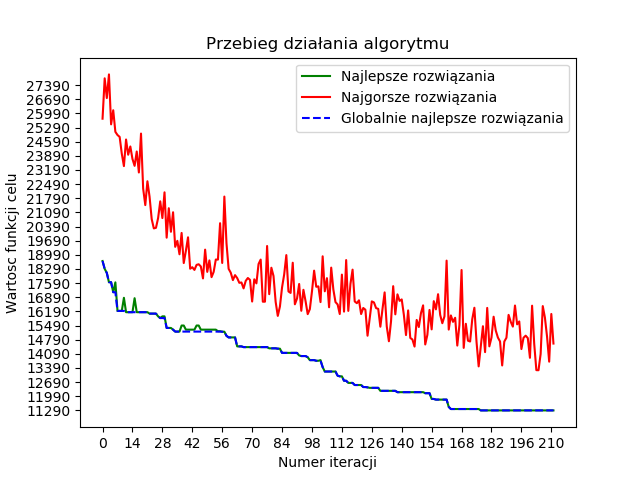
\includegraphics{punkt_odniesienia.png}
\end{figure}
\par
Następnie zmieniliśmy rodzaj sukcesji na mieszaną, to znaczy że do następnej generacji mogli przejść zarówno rodzice jak i dzieci. Wyniki przedstawiamy w tabeli 7.
\begin{table}[H]
\caption{Wyniki testów dla sukcesji mieszanej}
\begin{center}
\scalebox{0.8}{
\begin{tabular}{|c|c|c|c|c|c|c|c|c|c|c|}
\hline
L. iteracji & 320 & 400 & 700 & 383 & 264 & 234 & 413 & 250 & 383 & 271 \\ \hline
Wart. naj. rozw. & 11232 & 11162 & 10472 & 10350 & 10784 & 11422 & 11116 & 10624 & 11102 & 10678\\ \hline
\end{tabular}}
\end{center}
\end{table}
Średnia najlepszych wartości funkcji celu wyniosła 10894.2, a ich odchylenie standardowe wyniosło 359.49. Średnia ilość iteracji wyniosła 361. Wartość średnia poprawiła się, odchylenie standardowe również zmniejszyło się, to znaczy że otrzymywaliśmy bardziej zbliżone do siebie i wartości średniej wyniki. Widać to również na wykresie - otrzymywane populacje miały bardziej zbliżone do siebie wartości funkcji celu, gdyż odległości pomiędzy punktami oznaczającymi wartości najlepszych i najgorszych rozwiązań zmniejszyły się. Przykładowy przebieg działania algorytmu znajduje się na wykresie 3.
\begin{figure}[H]
\caption{Przebieg działania algorytmu dla sukcesji mieszanej}
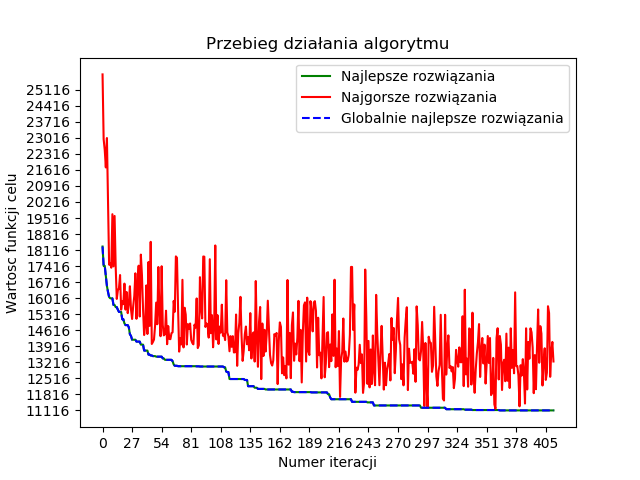
\includegraphics{mixed_succession3.png}
\end{figure}
\par
Następnie względem parametrów z tabeli 5 zmieniliśmy rozmiar turnieju na 8. Wyniki testów przedstawiamy w tabeli 8.
\begin{table}[H]
\caption{Wyniki testów dla selekcji turniejowej o rozmiarze turnieju 8}
\begin{center}
\scalebox{0.8}{
\begin{tabular}{|c|c|c|c|c|c|c|c|c|c|c|}
\hline
L. iteracji & 335 & 431 & 355 & 224 & 212 & 385 & 320 & 493 & 625 & 320 \\ \hline
Wart. naj. rozw. & 11164 & 11602 & 11460 & 11626 & 11290 & 11436 & 11516 & 10790 & 11002 & 12595 \\ \hline
\end{tabular}}
\end{center}
\end{table}
Średnia wartości najlepszych rozwiązań pogorszyła się, bo wynosiła 11448.1, a odchylenie standardowe wynosiło 484.59. Średnia liczba iteracji wyniosła 370. Zmniejszając jeszcze bardziej rozmiar turnieju do 4 otrzymaliśmy wyniki zamieszczone w tabeli 9.
\begin{table}[H]
\caption{Wyniki testów dla selekcji turniejowej o rozmiarze turnieju 4}
\begin{center}
\scalebox{0.8}{
\begin{tabular}{|c|c|c|c|c|c|c|c|}
\hline
L. iteracji & 727 & 994 & 1138 & 686 & 473 & 423 & 583 \\ \hline
Wart. naj. rozw. & 13608 & 12920 & 13338 & 13266 & 14604 & 14528 & 13300 \\ \hline
\end{tabular}}
\end{center}
\end{table}
Średnia wartości najlepszych rozwiązań wyniosła 13652, odchylenie standardowe wyniosło 656.12 a średnia liczba iteracji 717.  Z wykresu 4 widać, że zmniejszając rozmiar turnieju, osobnicy o najlepszej wartości funkcji celu częściej nie przechodzili do następnych generacji.
\begin{figure}[H]
\caption{Przebieg działania algorytmu dla selekcji turniejowej o rozmiarze turneiju 4}
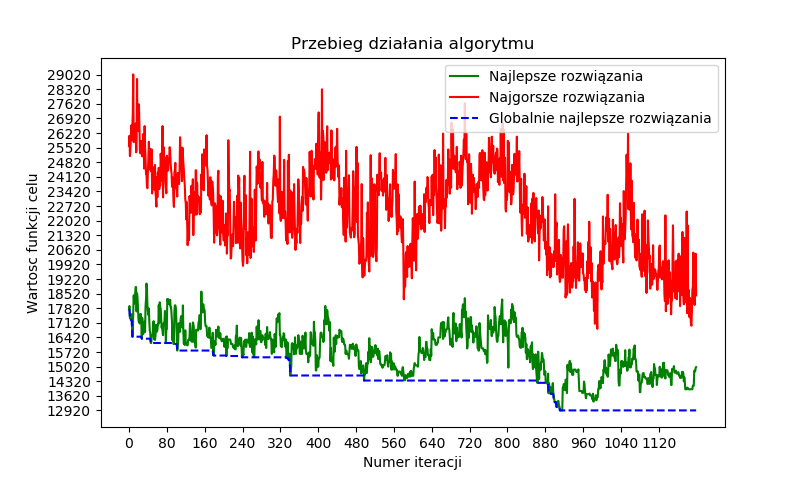
\includegraphics[scale=0.8]{tournament_size=4.png}
\end{figure}
\par
Następnie zmieniliśmy rodzaj selekcji na proporcjonalny względem parametrów z tabeli 5, z liczbą rodziców równą 20. Otrzymane wyniki przedstawiamy w tabeli 10.
\begin{table}[H]
\caption{Wyniki testów dla selekcji proporcjonalnej}
\begin{center}
\scalebox{0.8}{
\begin{tabular}{|c|c|c|c|c|c|c|c|}
\hline
L. iteracji &1009 & 1270 & 1018 & 1499 & 701 & 1350 & 1390 \\ \hline
Wart. naj. rozw. & 12020 & 11324 & 11468 & 12286 & 11654 & 11354 & 11020 \\ \hline
\end{tabular}}
\end{center}
\end{table}
Średnia wartości najlepszych rozwiązań wyniosła 11589.43, ich odchylenie standardowe wyniosło 435.82, a średnia liczba iteracji wyniosła 1176. Na wykresie 5 zamieszczamy przebieg działania algorytmu. Widać z niego, że mimo iż preferowane do selekcji są rozwiązania o lepszych wartościach funkcji celu, to nie koniecznie przejdą one do następnej populacji.
\begin{figure}[H]
\caption{Przebieg działania algorytmu dla selekcji proporcjonalnej}
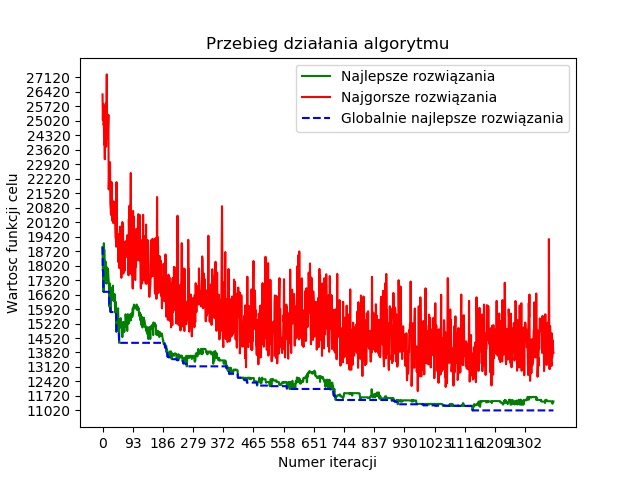
\includegraphics[scale=1]{proportionate=20_v4.png}
\end{figure}
\par
Po raz kolejny zmieniliśmy rodzaj selekcji, tym razem na odcinającą, co oznacza że wybieraliśmy tylko kilku najlepszych osobników z danej populacji rodziców, w naszym przypadku 30. Wyniki tego eksperymentu znajdują się w tabeli 11.
\begin{table}[H]
\caption{Wyniki testów dla selekcji odcinającej}
\begin{center}
\scalebox{0.8}{
\begin{tabular}{|c|c|c|c|c|c|c|c|}
\hline
L. iteracji & 437 & 515 & 667 & 441 & 477 & 415 & 547 \\ \hline
Wart. naj. rozw. & 10128 & 10094 & 10236 & 10888 & 10678 & 10732 & 10298 \\ \hline
\end{tabular}}
\end{center}
\end{table}
Średnia wartości najlepszych rozwiązań wyniosła 10436.29, ich odchylenie standardowe wyniosło 321.81, a średnia liczba iteracji wyniosła 499. Są to najlepsze do tej pory uzyskane przez nas wyniki. Przebieg działania algorytmu dla tych parametrów znajduje się na wykresie 6. Na wykresie wyraźnie widać, że najlepsi osobnicy zawsze przechodzili do następnej populacji.
\begin{figure}[H]
\caption{Przebieg działania algorytmu dla selekcji odcinającej}
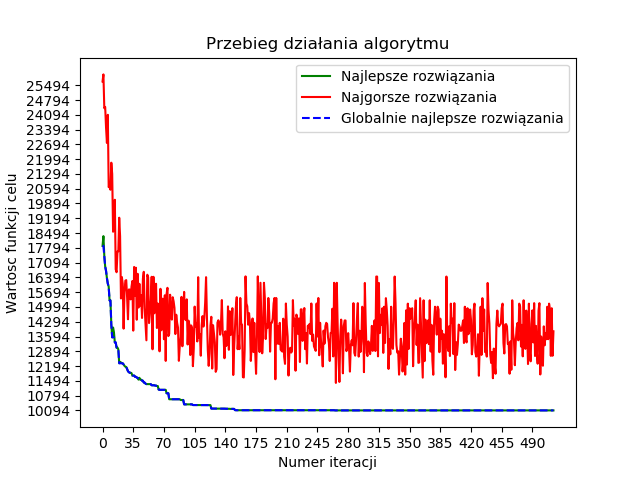
\includegraphics[scale=1]{truncation=30.png}
\end{figure}
\par
Następnie względem parametrów z tabeli 5, ustawiliśmy prawdopodobieństwo mutacji na 0. Otrzymane wyniki zamieściliśmy w tabeli 12.
\begin{table}[H]
\caption{Wyniki testów dla algorytmu bez mutacji}
\begin{center}
\scalebox{0.8}{
\begin{tabular}{|c|c|c|c|c|c|c|c|}
\hline
L. iteracji & 261 & 266 & 266 & 257 & 266 & 273 & 262 \\ \hline
Wart. naj. rozw. & 16186 & 14644 & 16394 & 15998 & 16040 & 14774 & 16020 \\ \hline
\end{tabular}}
\end{center}
\end{table}
Uniemożliwiając mutacje, otrzymaliśmy najgorsze do tej pory wyniki. Średnia wartości najlepszych wyników wyniosła 15722.29, a ich odchylenie standardowe wyniosło 706.37. Średnia ilość iteracji wyniosła 264. Oznacza to, że algorytm dość szybko wpadał w minimum lokalne i ze względu na brak mutacji nie dochodziło do dalszego przeszukiwania przestrzeni rozwiązań. Na tym przykładzie widać, jak ważna jest odpowiednia losowość podczas stosowania algorytmów genetycznych. Szybkie wpadnięcie w minimum lokalne widać też dobrze na przebiegu działania algorytmu znajdującym się na wykresie 7.
\begin{figure}[H]
\caption{Przebieg działania algorytmu bez mutacji}
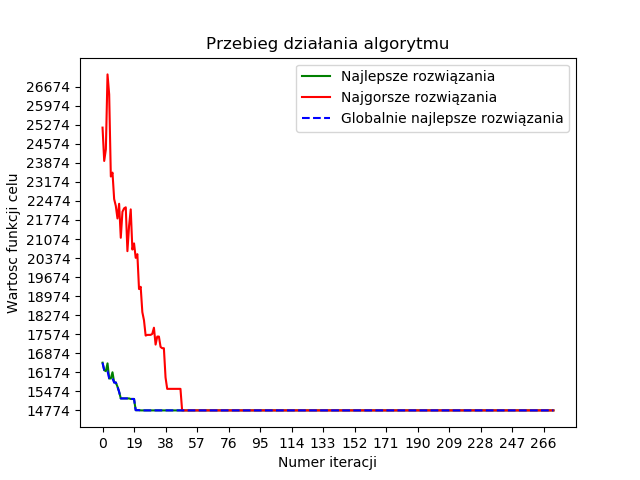
\includegraphics[scale=1]{no-mutation_v3.png}
\end{figure}
\par
Zamieniając względem parametrów z tabeli 5 mutację na inwersję z prawdopodobieństwem 30\% oraz wpływem o wartości 30\% na rozwiązanie, uzyskaliśmy znaczącą poprawę wyników w stosunku do przypadku, w którym mutacje były niemożliwe. Wyniki działania algorytmów z tymi parametrami przedstawiamy w tabeli 13.
\begin{table}[H]
\caption{Wyniki testów dla algorytmu z inwersją z prawdopodobieństwem 30\% i wpływem na rozwiązanie o wartości 30\%}
\begin{center}
\scalebox{0.8}{
\begin{tabular}{|c|c|c|c|c|c|c|c|}
\hline
L. iteracji & 838 & 859 & 893 & 883 & 538 & 519 \\ \hline
Wart. naj. rozw. & 10824 & 10408 & 10840 & 11090 & 11012 & 11126 \\ \hline
\end{tabular}}
\end{center}
\end{table}
Średnia wartości najlepszych rozwiązań wyniosła 10883.33, odchylenie standardowe wyniosło 264.38, a średnia liczba iteracji wyniosła 755. Przykładowy przebieg działania algorytmu dla tych parametrów znajduje się na wykresie 8. Widać także po wartościach najlepszych i najgorszych rozwiązań w danej iteracji, że przestrzeń rozwiązań była dokładniej przeszukiwana, a populacje były bardziej różnorodne.
\begin{figure}[H]
\caption{Przebieg działania algorytmu z inwersją z prawdopodobieństwem 30\% i wpływem na rozwiązanie o wartości 30\%}
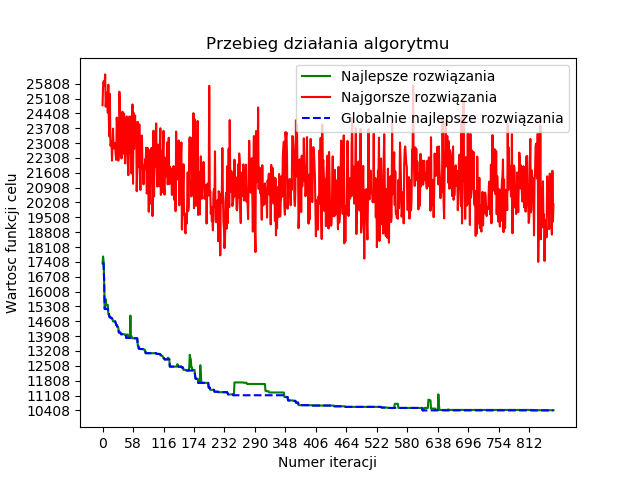
\includegraphics[scale=1]{inversion_30_percent_v2.png}
\end{figure}
\par
Przebadaliśmy również działanie operatora OX. Dawał on bardzo podobne wyniki do operatora PMX co może oznaczać, że zachowanie względnej kolejności podciągów rozwiązania nie jest zbyt istotne w rozważanym przez nas problemie. Po analizie zamieszczonych wyżej wyników, staraliśmy się dobrać parametry algorytmu tak, aby dawał jak najlepsze rozwiązania. Najlepsze rozwiązanie udało nam się uzyskać przy zastosowaniu operatora krzyżowania OX, selekcji odcinającej, zachowującej 30\% najlepszych osobników, mutacji swap o prawdopodobieństwie wystąpienia 30\% oraz sukcesji mieszanej. Po 609 iteracjach otrzymaliśmy rozwiązanie o wartości funkcji celu wynoszącej 9844, które różniło się już o bardzo niewiele wartości funkcji celu rozwiązania optymalnego. Przebieg działania algorytmu dla owych parametrów prezentujemy na wykresie 9.
\begin{figure}[H]
\caption{Przebieg działania algorytmu z dobranymi przez nas parametrami}
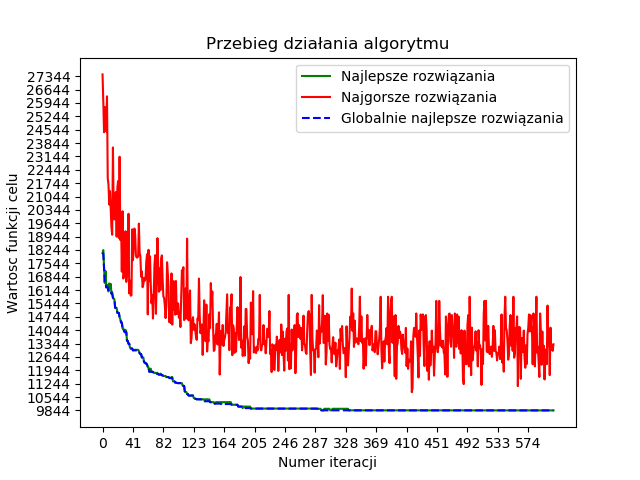
\includegraphics[scale=1]{experimental2_v2.png}
\end{figure}
\par
\section{Wnioski}
Podczas zajęć zapoznaliśmy się z różnymi algorytmami przybliżonymi. Sami zaimplementowaliśmy algorytm genetyczny w języku programowania Python oraz przetestowaliśmy jego działanie dla różnych parametrów. Idea jego działania inspirowana procesem ewolucji biologicznej jest dość prosta do zrozumienia oraz zaimplementowania, co czyni tę metodę potężnym narzędziem do rozwiązywania trudnych problemów optymalizacyjnych. Jednak aby efektywnie wykorzystać algorytm genetyczny należy pamiętać o odpowiedniej losowości, która jest jednym z ważniejszych czynników decydujących o skuteczności omawianej przez nas metody. Owa losowość w połączeniu z operatorami selekcji zapewniającymi większe szanse na przetrwanie lepiej przystosowanych osobników czyni algorytm genetyczny funkcjonalnym. Podczas testów mogliśmy się przekonać, że największym ograniczeniem przy rozwiązywaniu problemu QAP jest czas potrzebny na obliczanie funkcji celu. Bardzo ważne jest także dobre zrozumienie rozważanego problemu pozwalające na odpowiednie dobranie parametrów algorytmu.
\end{document}